\begin{figure}
    \centering
    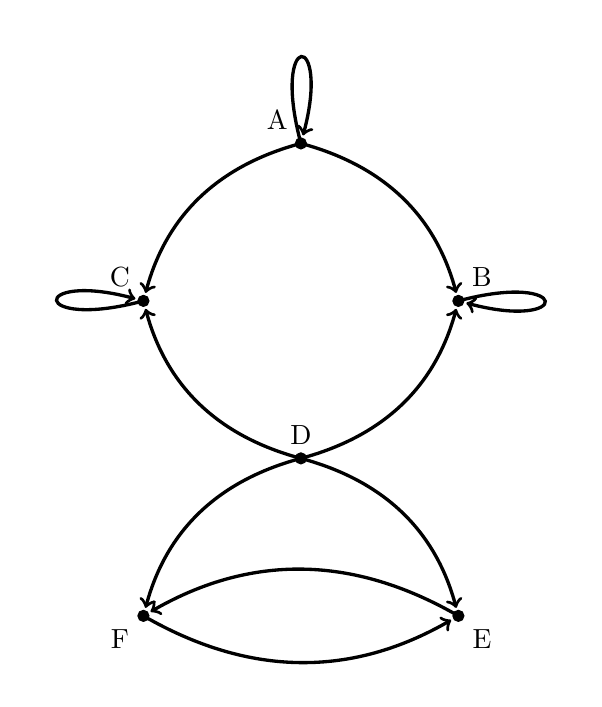
\begin{tikzpicture}

%% vertices
\draw[fill=black] (2,6) circle (2pt);   %% a
\draw[fill=black] (0,4) circle (2pt);   %% b
\draw[fill=black] (4,4) circle (2pt);   %% c
\draw[fill=black] (2,2) circle (2pt);   %% d
\draw[fill=black] (0,0) circle (2pt);   %% e
\draw[fill=black] (4,0) circle (2pt);   %% f

%% vertex labels
\node at (1.7,6.3) {A};
\node at (-0.3,4.3) {C};
\node at (4.3,4.3) {B};
\node at (2,2.3) {D};
\node at (-0.3,-0.3) {F};
\node at (4.3,-0.3) {E};

%%% edges
\draw[-{>[sep=3pt]}, very thick] (2,6) to [loop above, min distance=1.5cm] (2,6);     %% aa
\draw[-{>[sep=3pt]}, very thick] (2,6) to [bend right] (0,4);     %% ab
\draw[-{>[sep=3pt]}, very thick] (0,4) to [loop left, min distance=1.5cm] (0,4);     %% bb
\draw[-{>[sep=3pt]}, very thick] (2,6) to [bend left] (4,4);     %% ac
\draw[-{>[sep=3pt]}, very thick] (4,4) to [loop right, min distance=1.5cm] (4,4); %% cc
\draw[-{>[sep=3pt]}, very thick] (2,2) to [bend right] (4,4); %% dc
\draw[-{>[sep=3pt]}, very thick] (2,2) to [bend left] (0,4);     %% db
\draw[-{>[sep=3pt]}, very thick] (2,2) to [bend right] (0,0);     %% de
\draw[-{>[sep=3pt]}, very thick] (2,2) to [bend left] (4,0);     %% df
\draw[-{>[sep=3pt]}, very thick] (0,0) to [bend right] (4,0);     %% ef
\draw[-{>[sep=3pt]}, very thick] (4,0) to [bend right] (0,0);     %% fe
    \end{tikzpicture}
    \label{q4-a}
    \caption{Isomorphism in quesrtion 4}
\end{figure}